\chapter{Example Results}
\begin{figure} \label{fig:singlecmaps}
	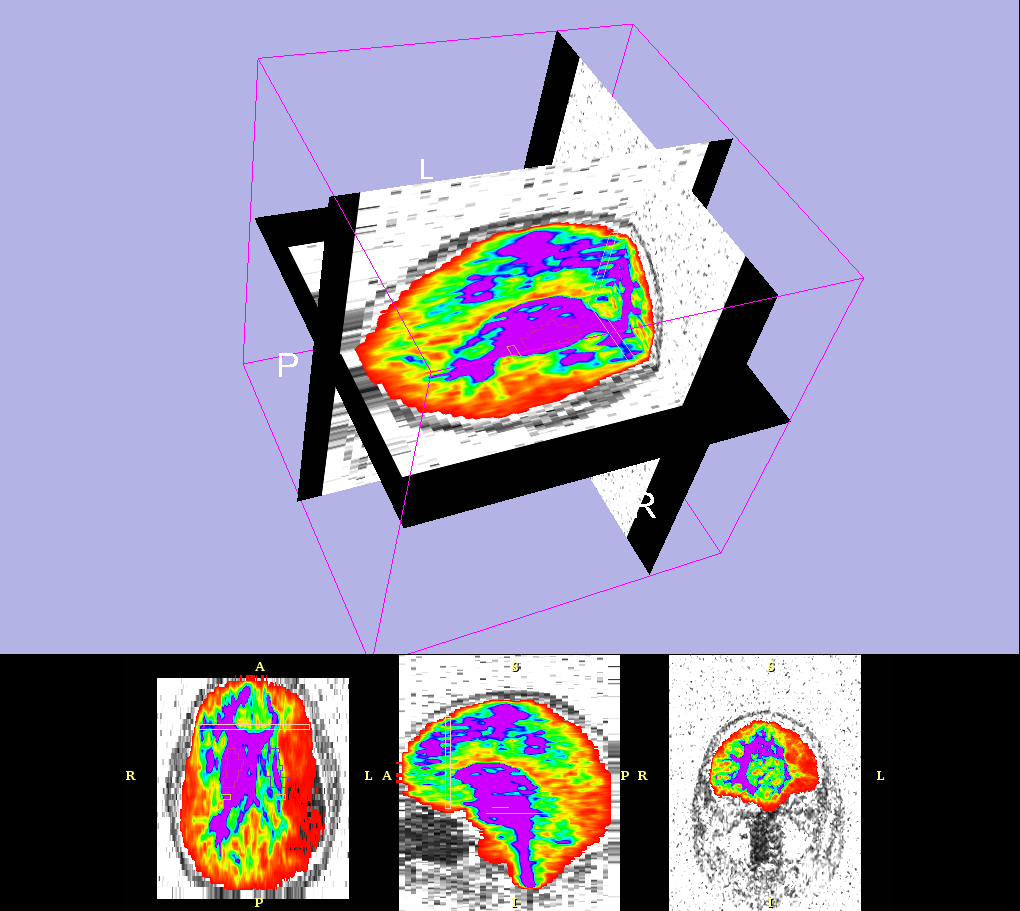
\includegraphics[width=0.5\linewidth]{slicer-0022}
	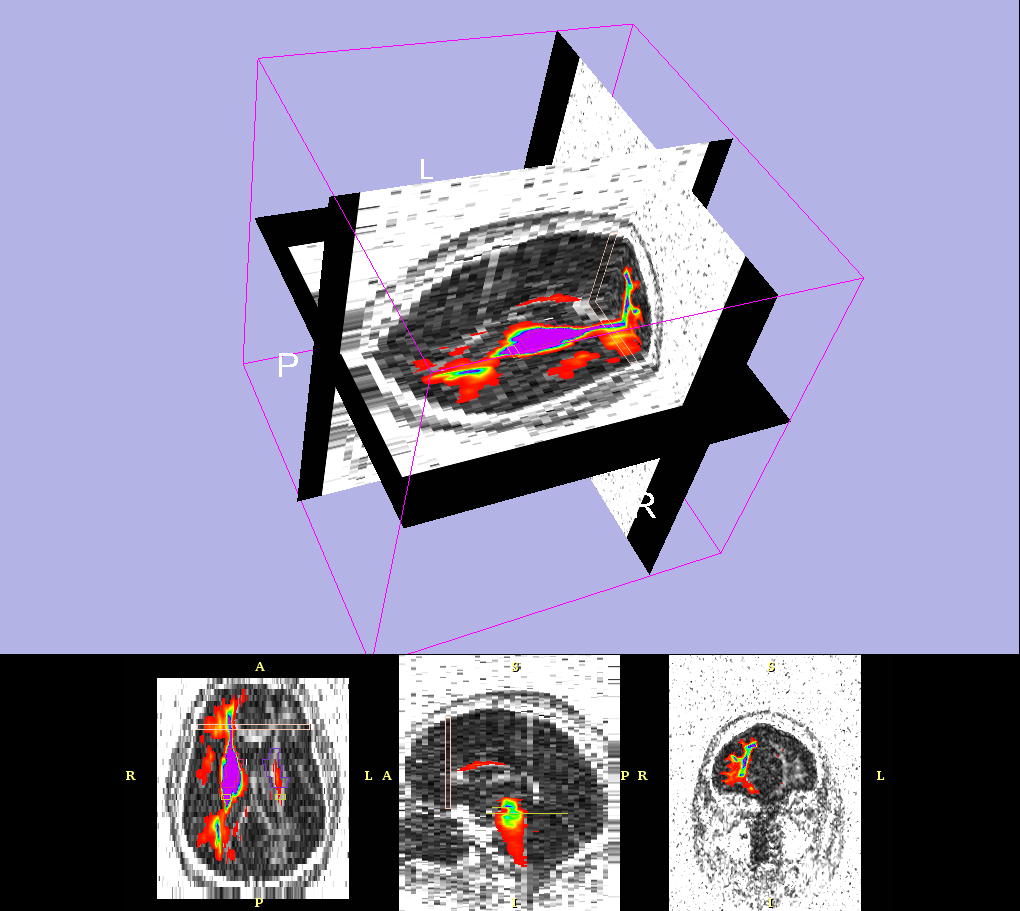
\includegraphics[width=0.5\linewidth]{slicer-0020}
	\caption{Connectivity maps of fibers which originate from the internal capsule.  The image on the left is without the use of a white matter posterior probability map.  The image on the right is with a white matter posterior probability map.  Notice that the reduced spatial variance of the fibers in the when using the white matter posterior.}
\end{figure}

\begin{figure} \label{fig:singleFAhistograms}
	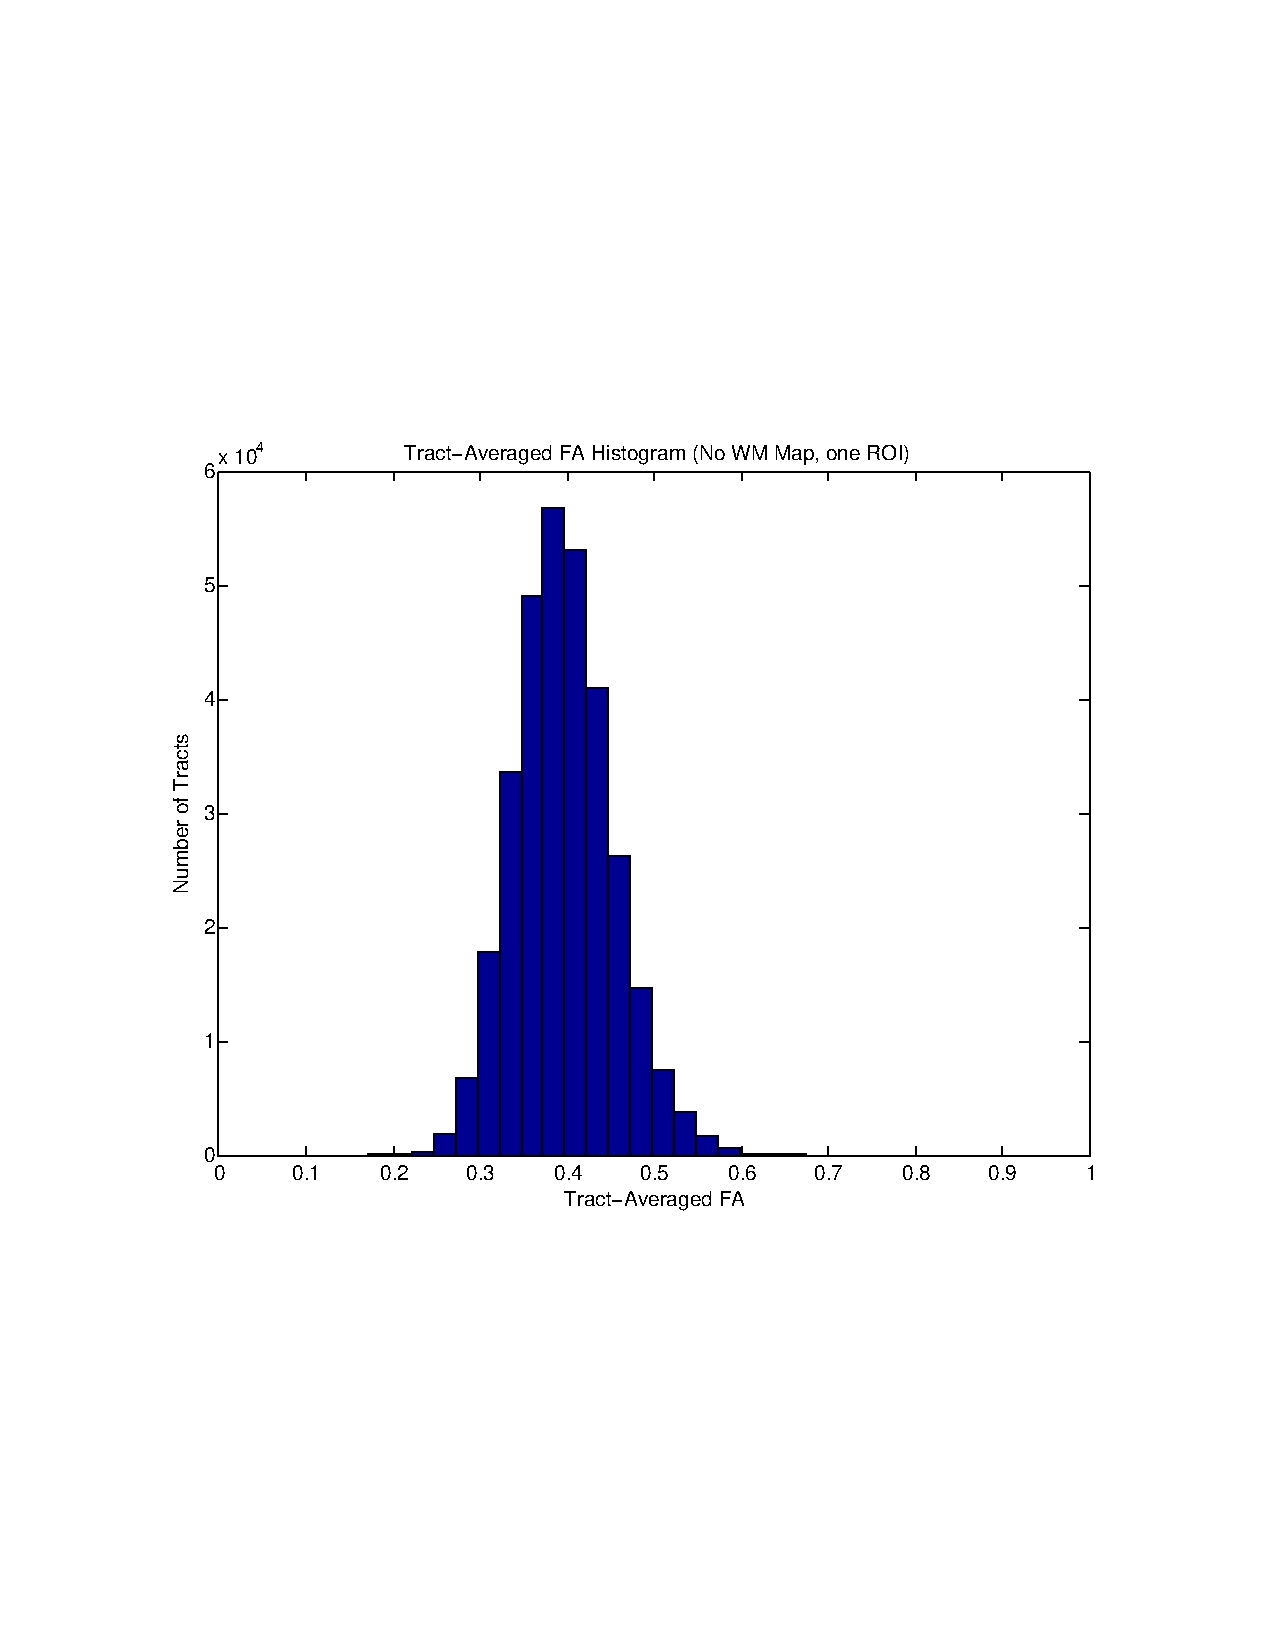
\includegraphics[trim = 20mm 70mm 20mm 70mm, clip, width=0.5\linewidth]
	  {hist_FA_nomask_single}
	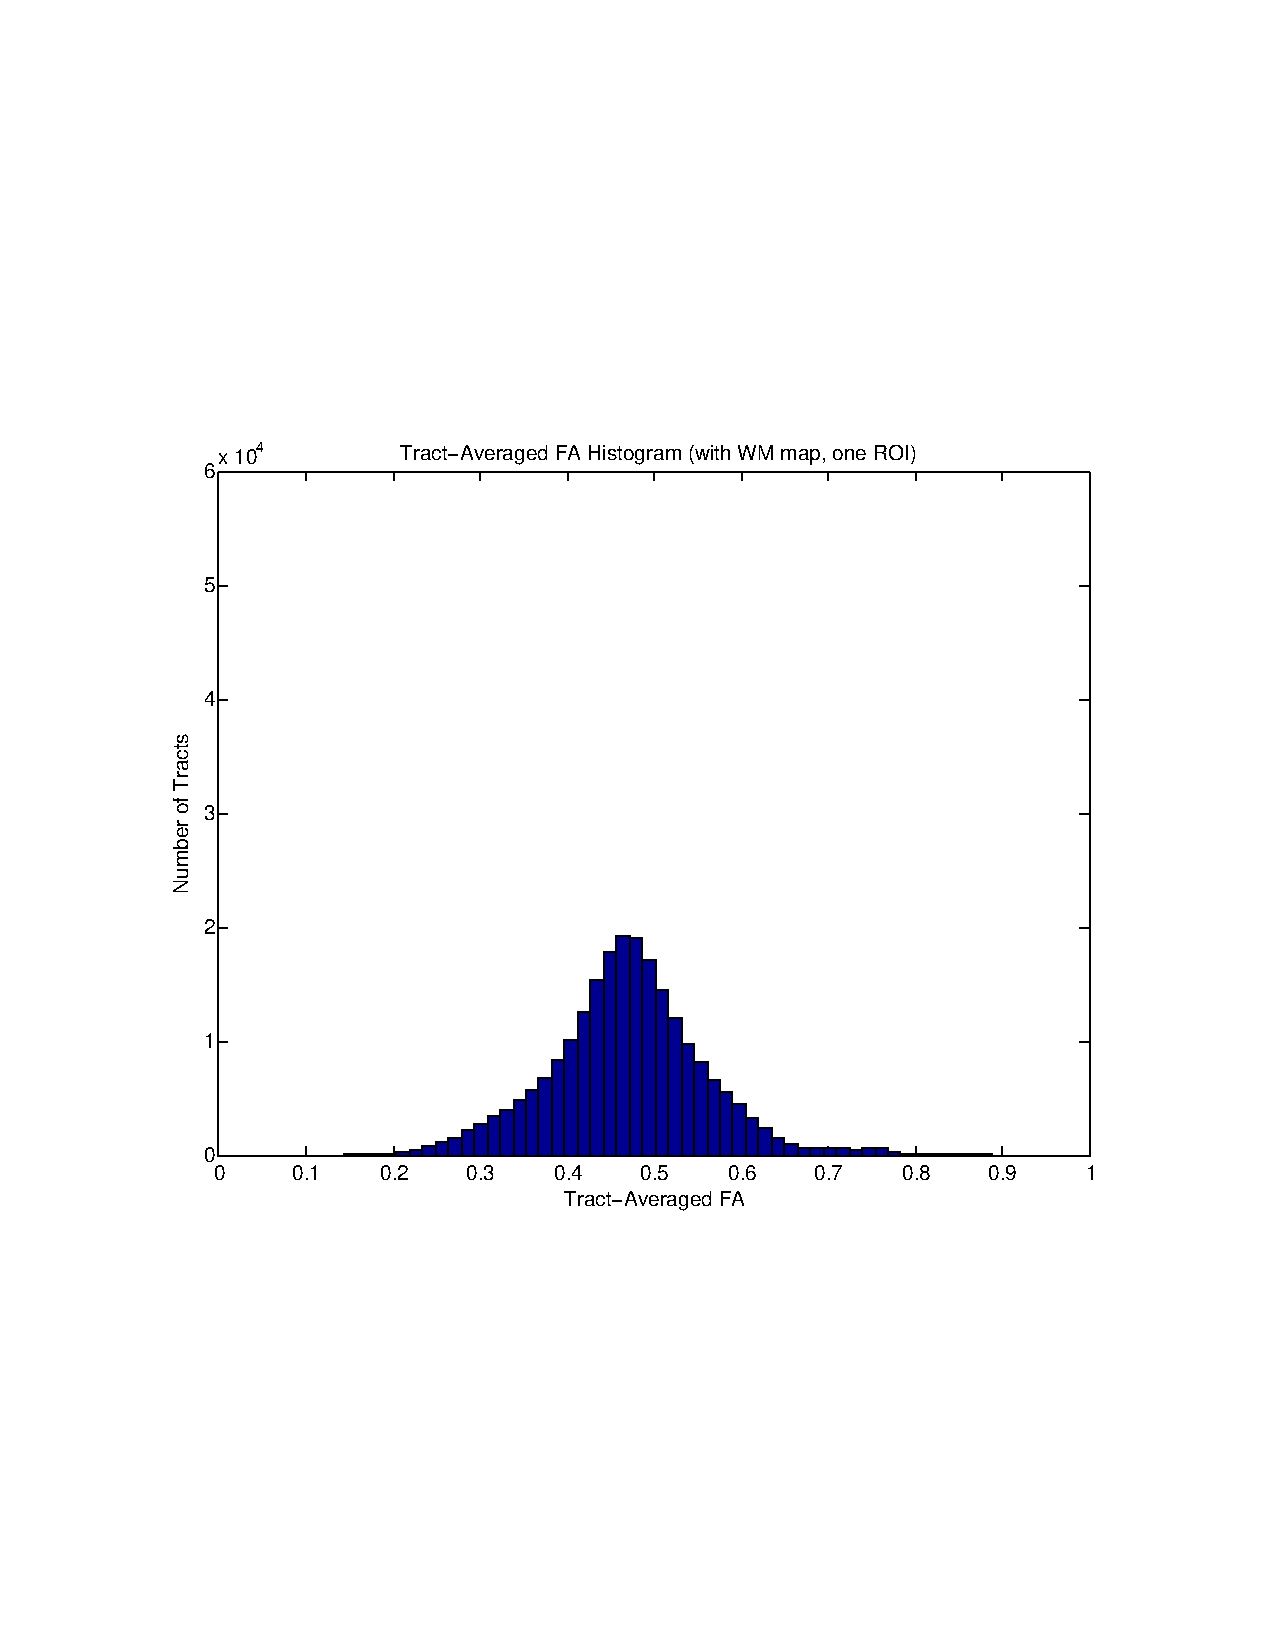
\includegraphics[trim = 20mm 70mm 20mm 70mm, clip, width=0.5\linewidth]
	  {hist_FA_mask_single}
	\caption{A histogram of tract-averaged Fractional Anisotropy.  Notice that using the white matter map increases the mean of the distribution, which is expected since we are no longer tracking in gray matter which has low anisotropy }
\end{figure}

\begin{figure} \label{fig:singelengthhistograms}
	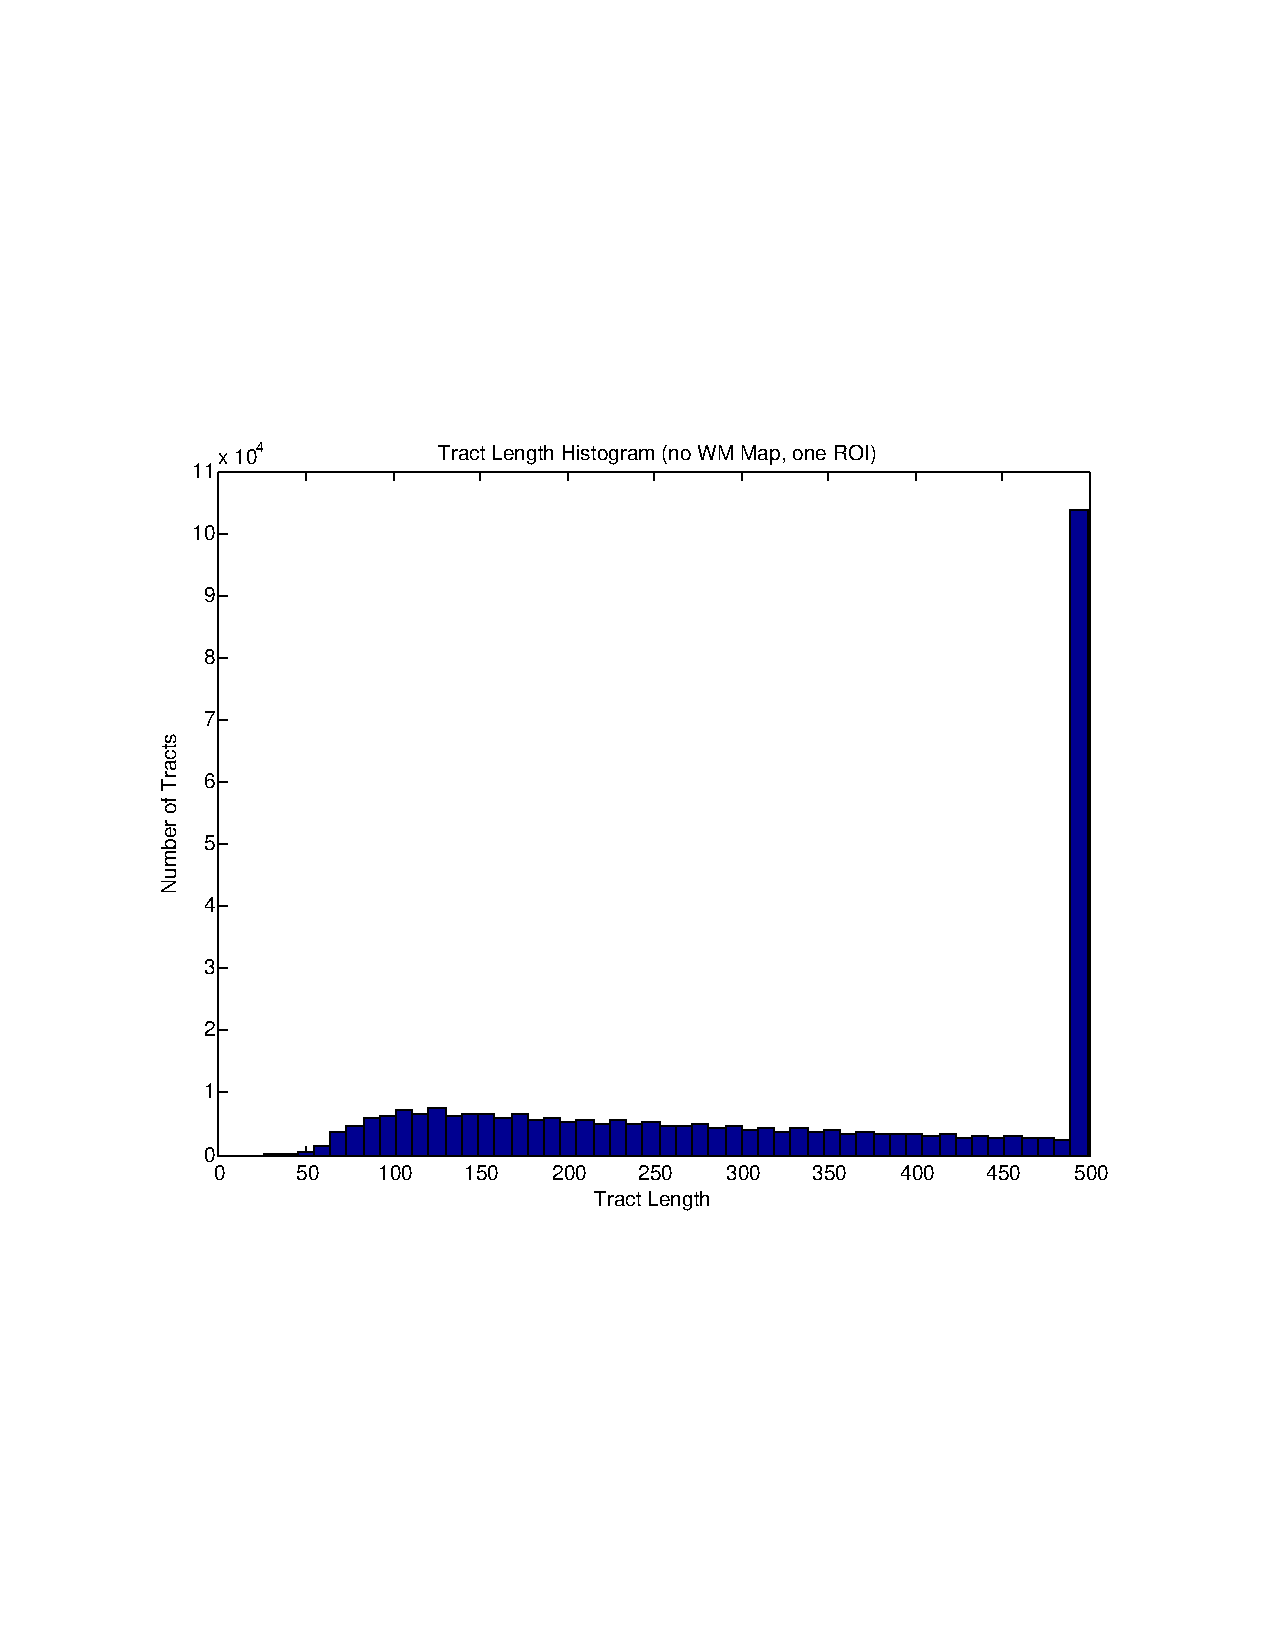
\includegraphics[trim = 20mm 70mm 20mm 70mm, clip, width=0.5\linewidth]
	  {hist_length_nomask_single}
	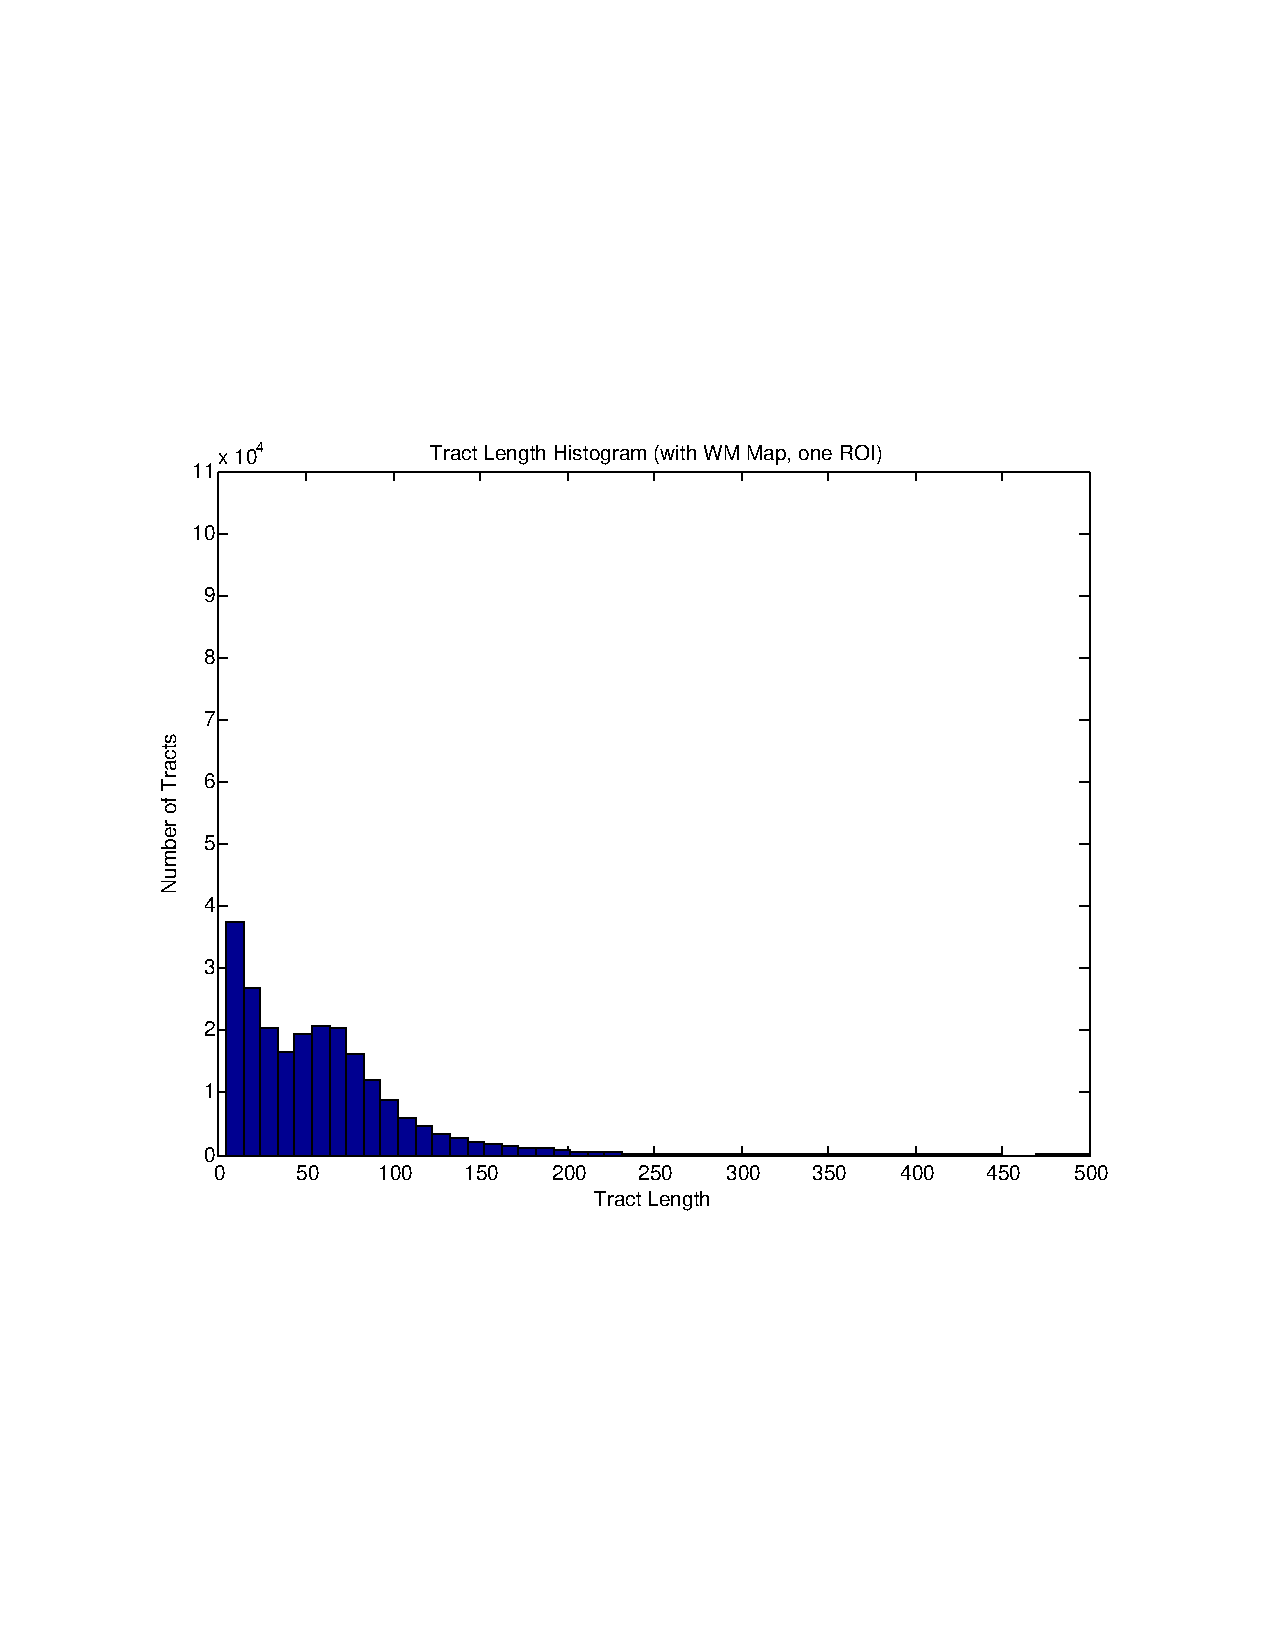
\includegraphics[trim = 20mm 70mm 20mm 70mm, clip, width=0.5\linewidth]
	  {hist_length_mask_single}
	\caption{A histogram of estimated fiber lengths.  The image on the left does not use a posterior white matter probability map while the one on the right does.  Notice that without the white matter posterior many fibers reach the arbitrary maximum tract limit of 500, providing little information about the actual distribution of tract lenghts.  With the white matter posterior probability map, the distribution of tract lengths is more plausible and few make it to the arbitrary 500 max length limit.}
\end{figure}

\begin{figure} \label{fig:twocmaps}
	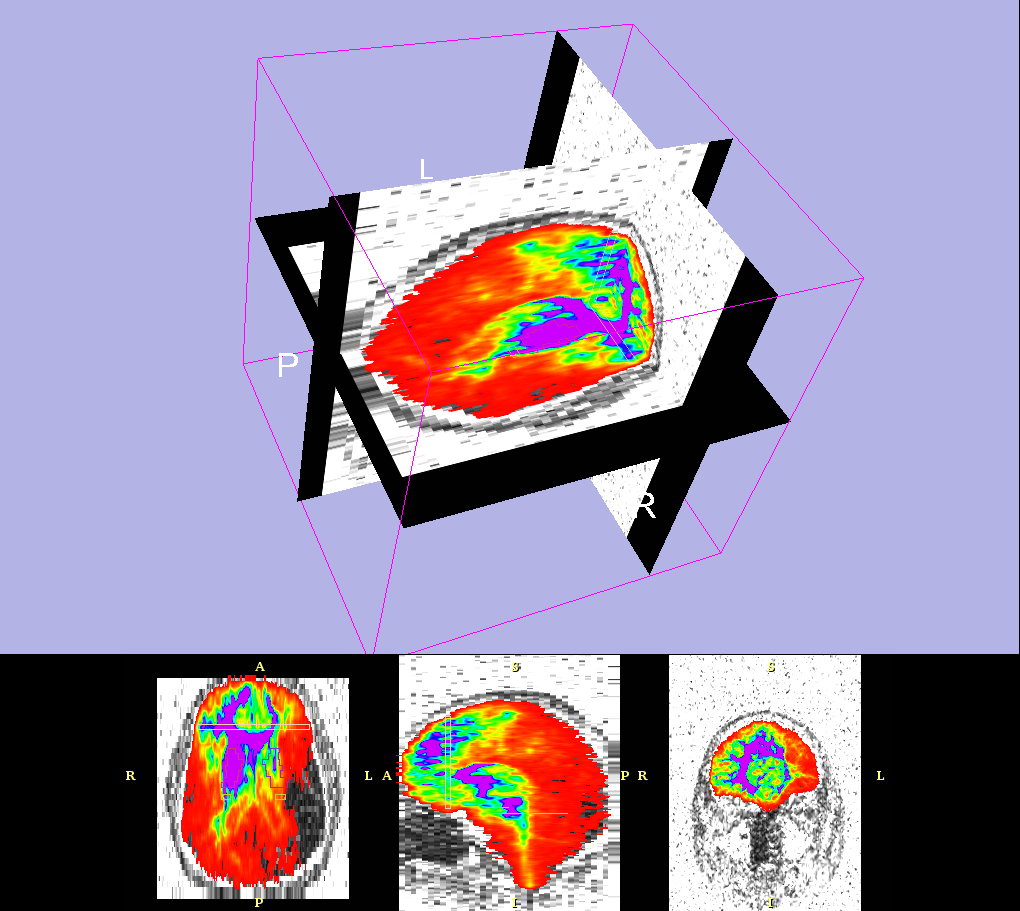
\includegraphics[width=0.5\linewidth]{slicer-0021}
	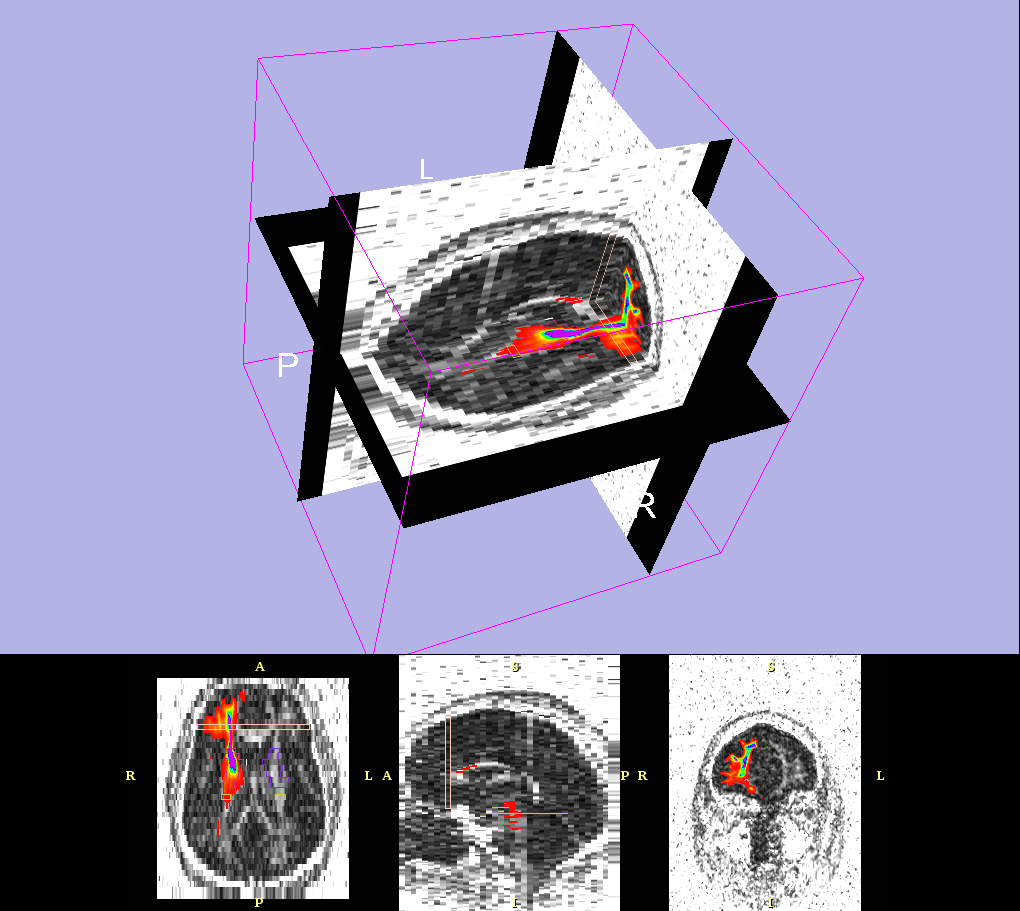
\includegraphics[width=0.5\linewidth]{slicer-0019}
	\caption{Connectivity maps of fibers which originate from the internal capsule and pass through a second region of interest placed in the frontal lobe.  The image on the left is without the use of a white matter posterior probability map.  The image on the right is with a white matter posterior probability map.  Notice that the reduced spatial variance of the fibers in the when using the white matter posterior.  Additionally, since we are excluding many tracts which don't pass through both ROI's, we have fewer samples.  Using the white matter posterior probability map the similar affect of reducing the number of acceptable sampels.}
\end{figure}

\begin{figure} \label{fig:twoFAhistograms}
	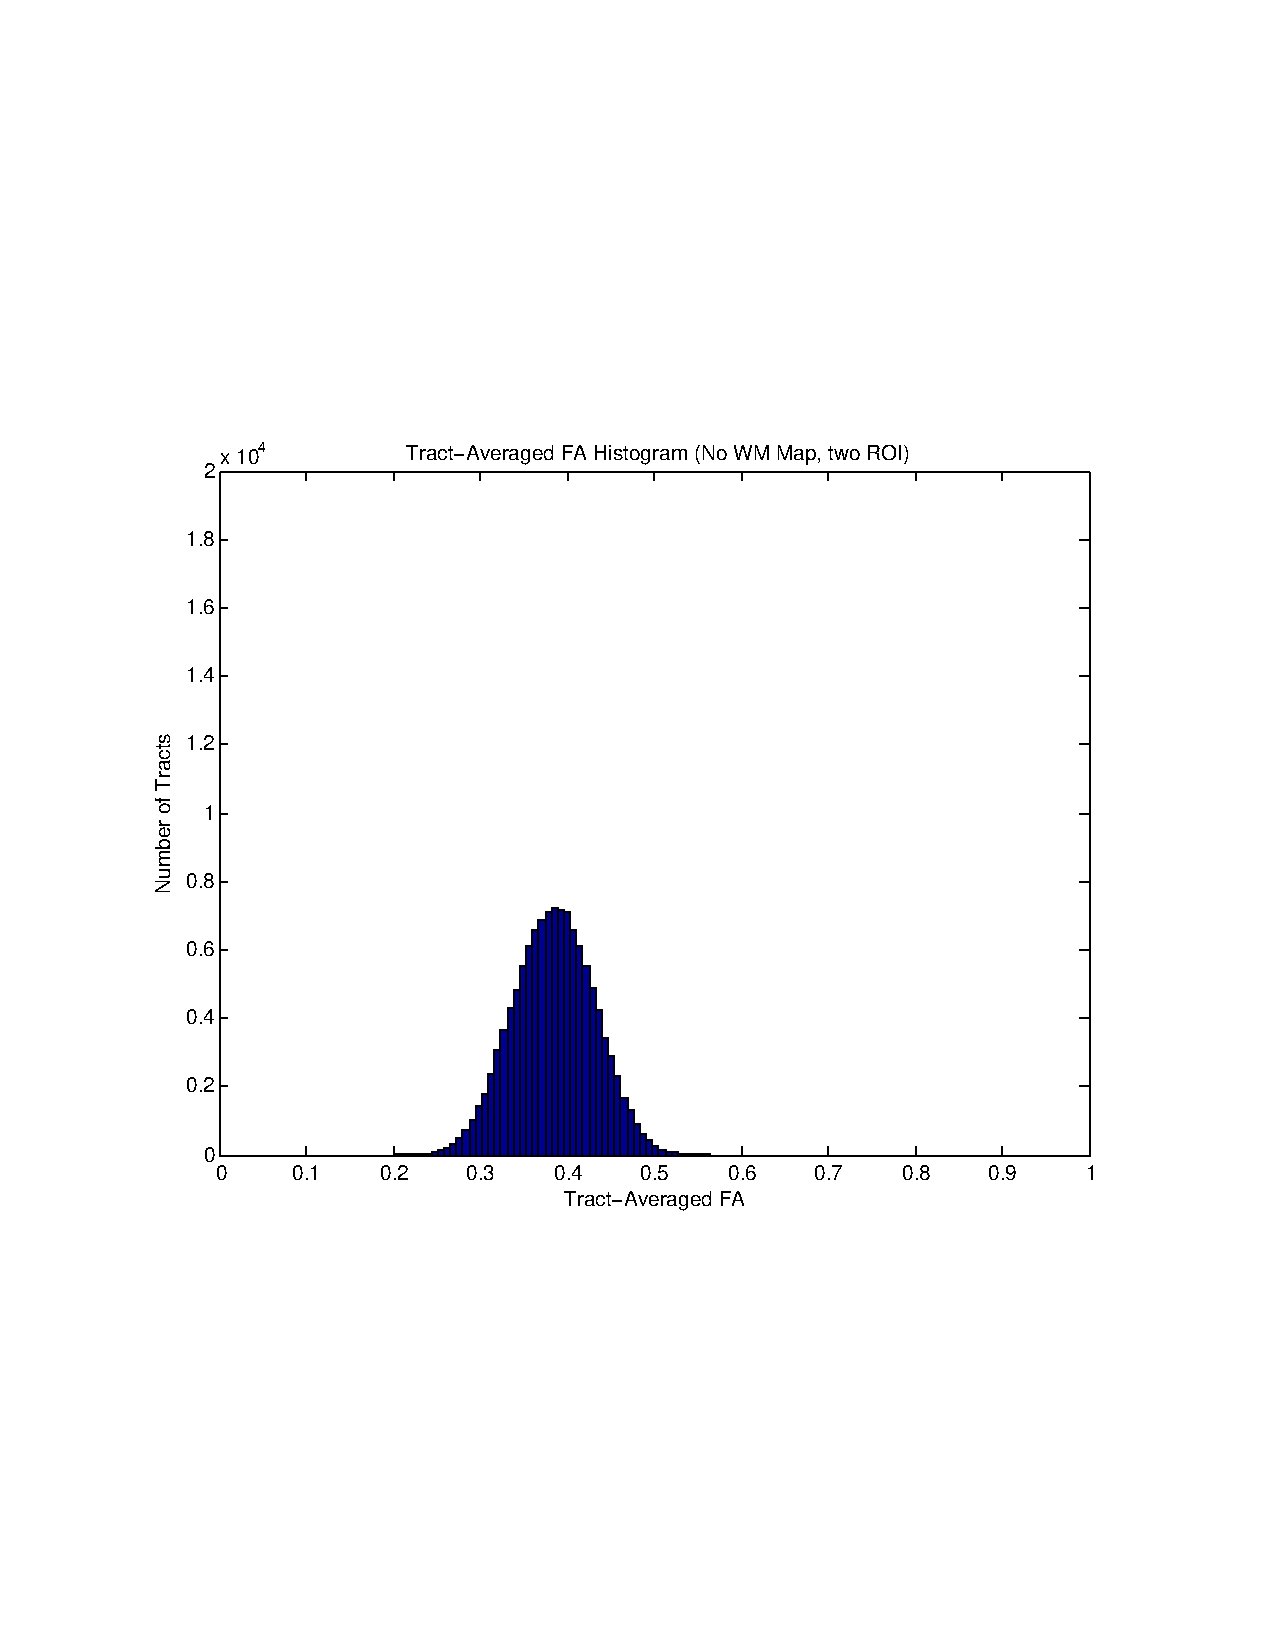
\includegraphics[trim = 20mm 70mm 20mm 70mm, clip, width=0.5\linewidth]
	  {hist_FA_nomask_two}
	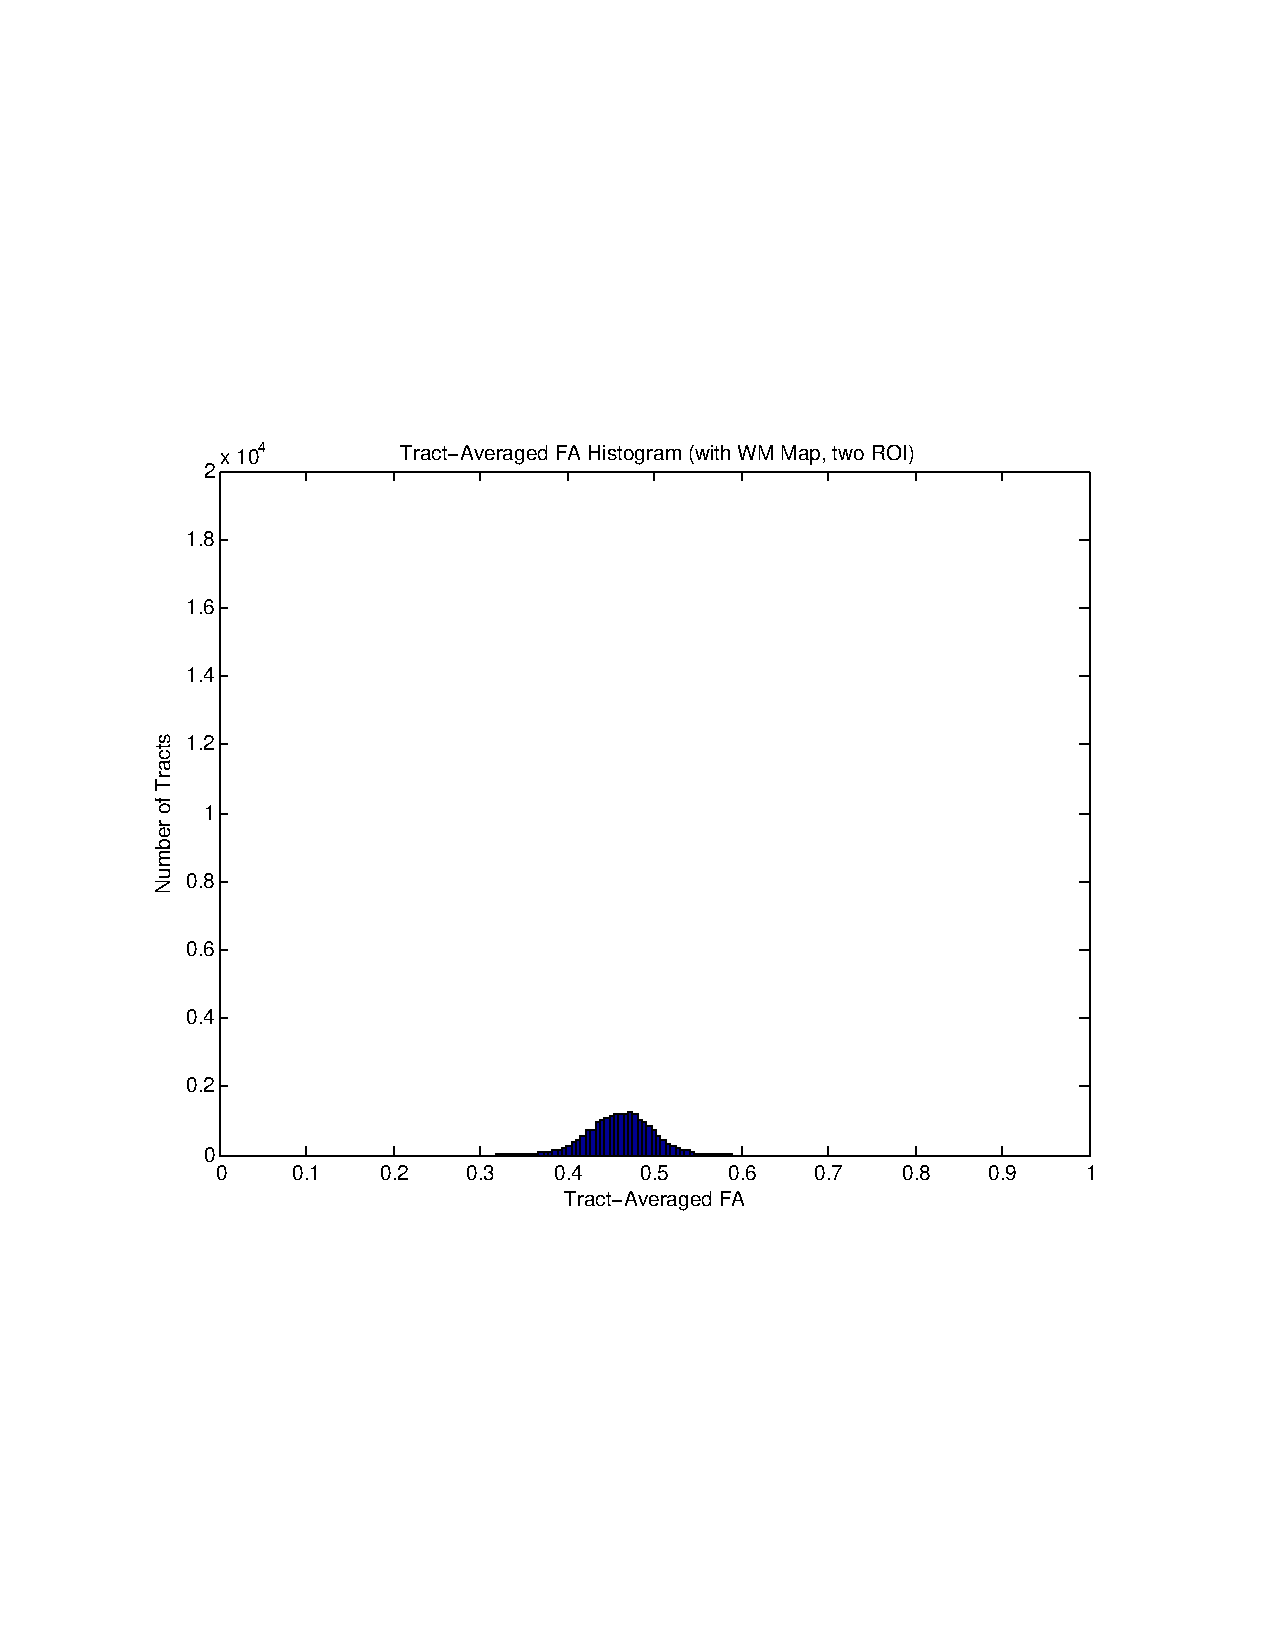
\includegraphics[trim = 20mm 70mm 20mm 70mm, clip, width=0.5\linewidth]
	  {hist_FA_mask_two}
	\caption{A histogram of tract-averaged Fractional Anisotropy.  Notice that using the white matter map increases the mean of the distribution, which is expected since we are no longer tracking in gray matter which has low anisotropy }
\end{figure}

\begin{figure} \label{fig:twolengthhistograms}
	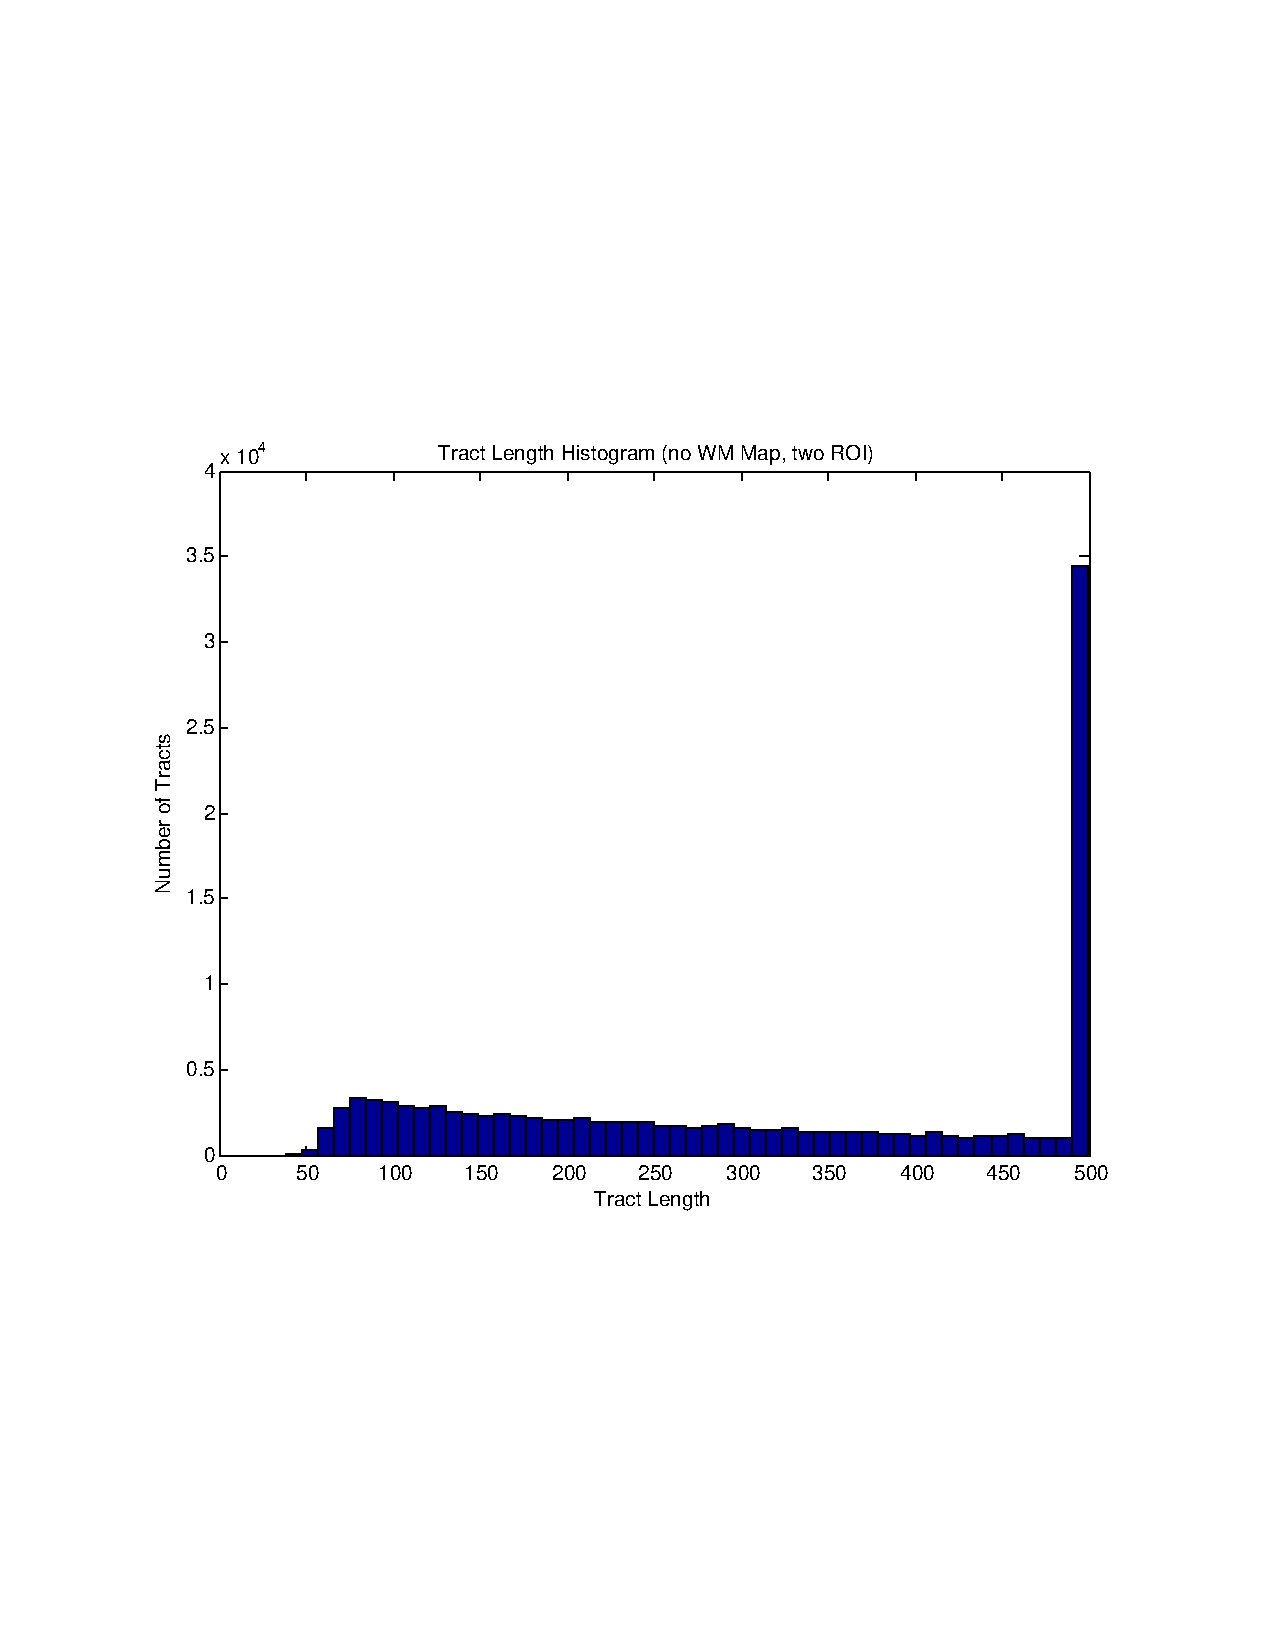
\includegraphics[trim = 20mm 70mm 20mm 70mm, clip, width=0.5\linewidth]
	  {hist_length_nomask_two}
	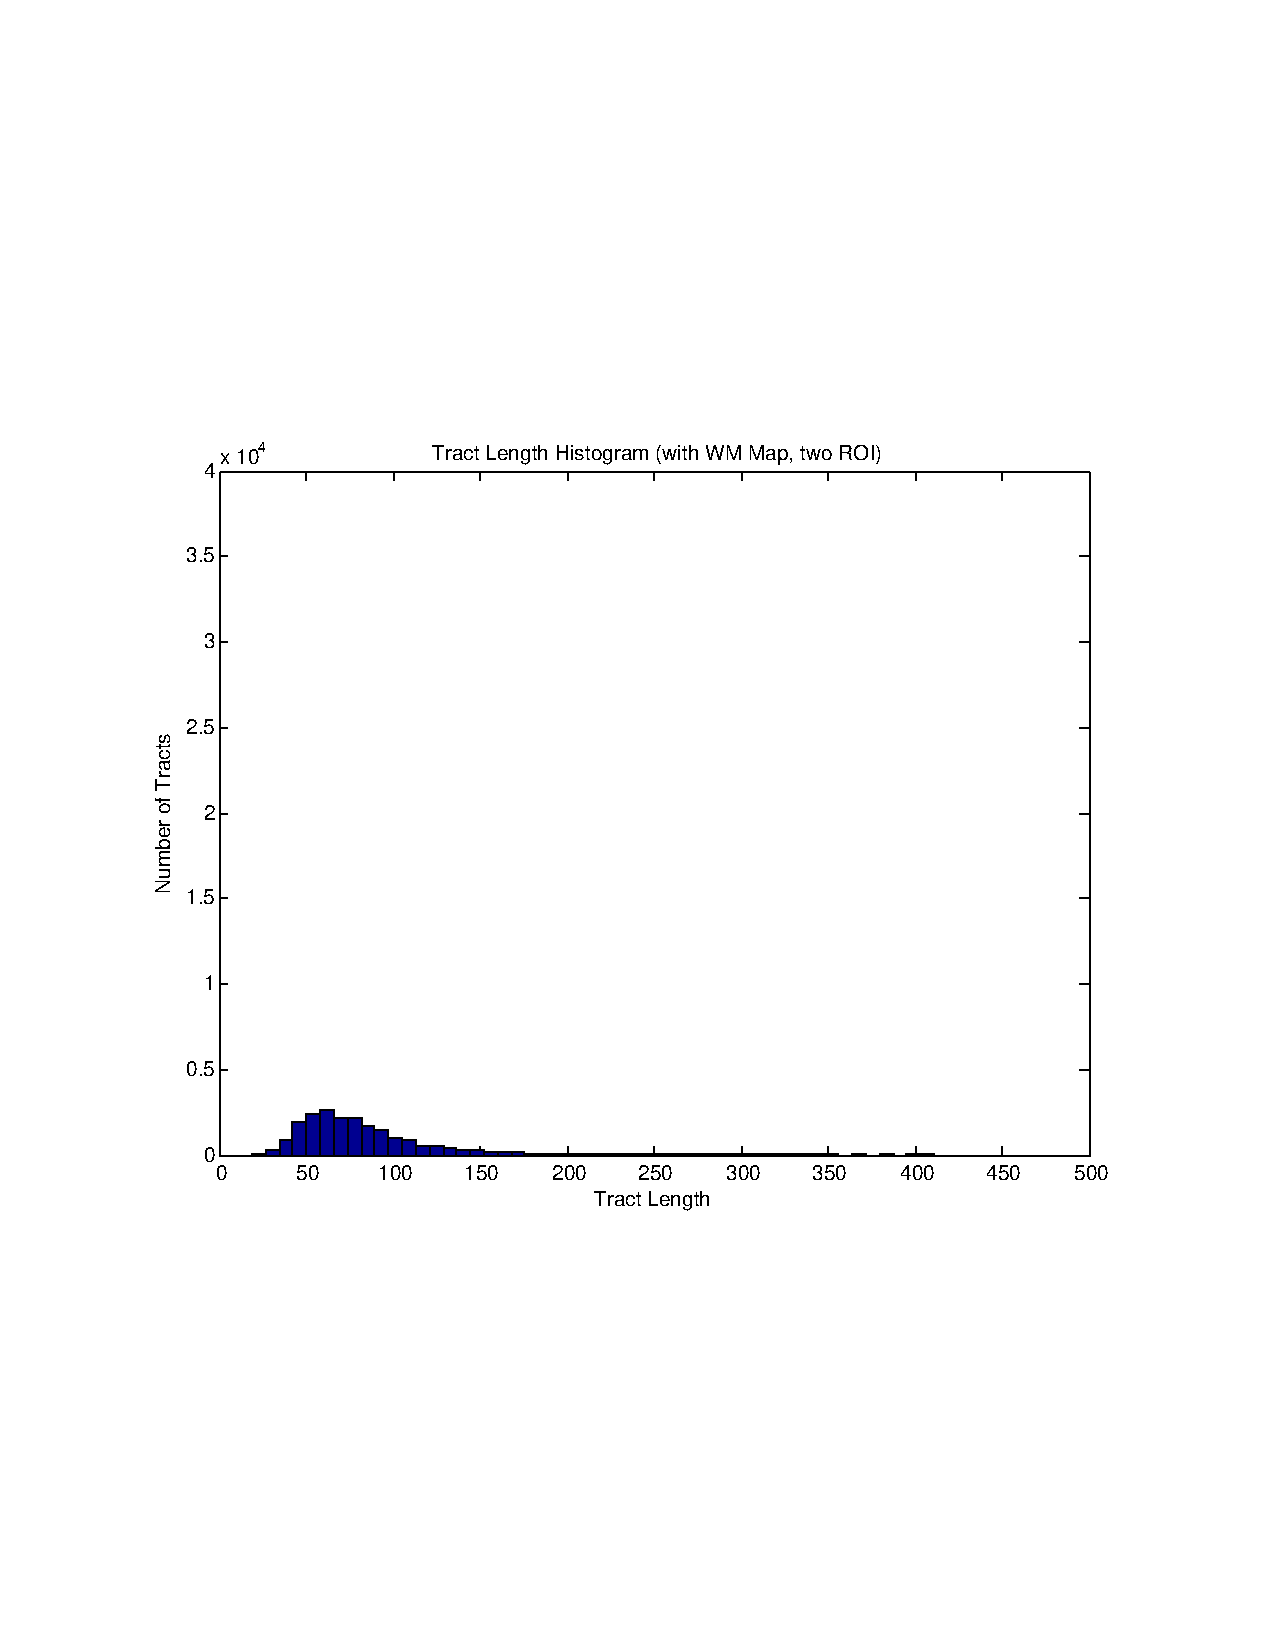
\includegraphics[trim = 20mm 70mm 20mm 70mm, clip, width=0.5\linewidth]
	  {hist_length_mask_two}
	\caption{A histogram of estimated fiber lengths.  The image on the left does not use a posterior white matter probability map while the one on the right does. }
\end{figure}

\section{Comparison with streamlining tractography}

\begin{figure} \label{fig:streamlinecomp}
	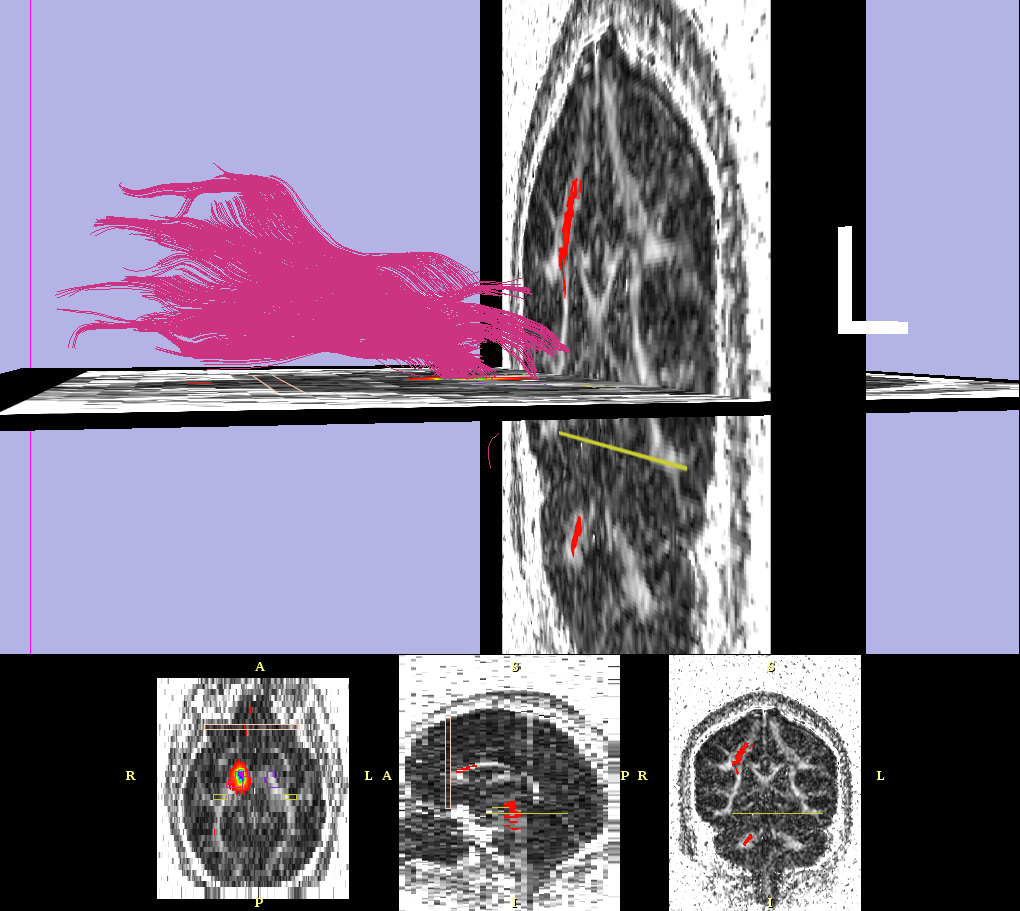
\includegraphics[width=0.5\linewidth]
	  {slicer-0016}
	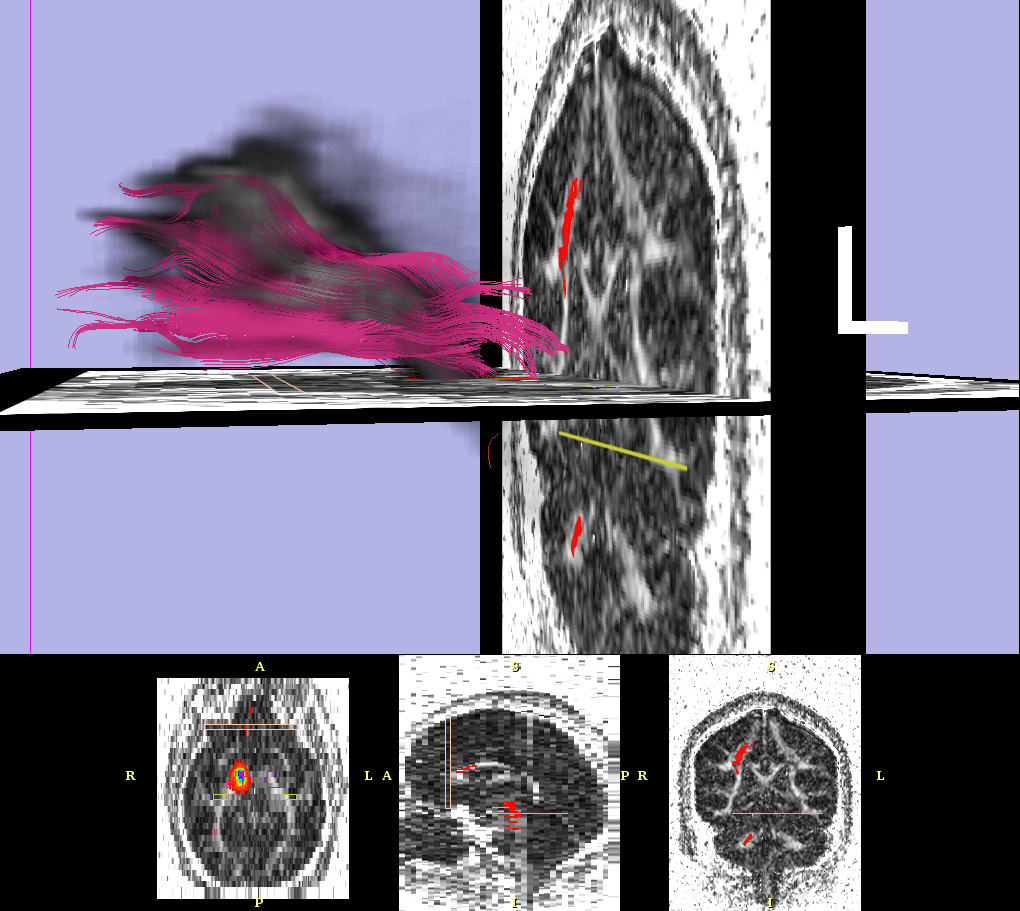
\includegraphics[width=0.5\linewidth]
	  {slicer-0015}
	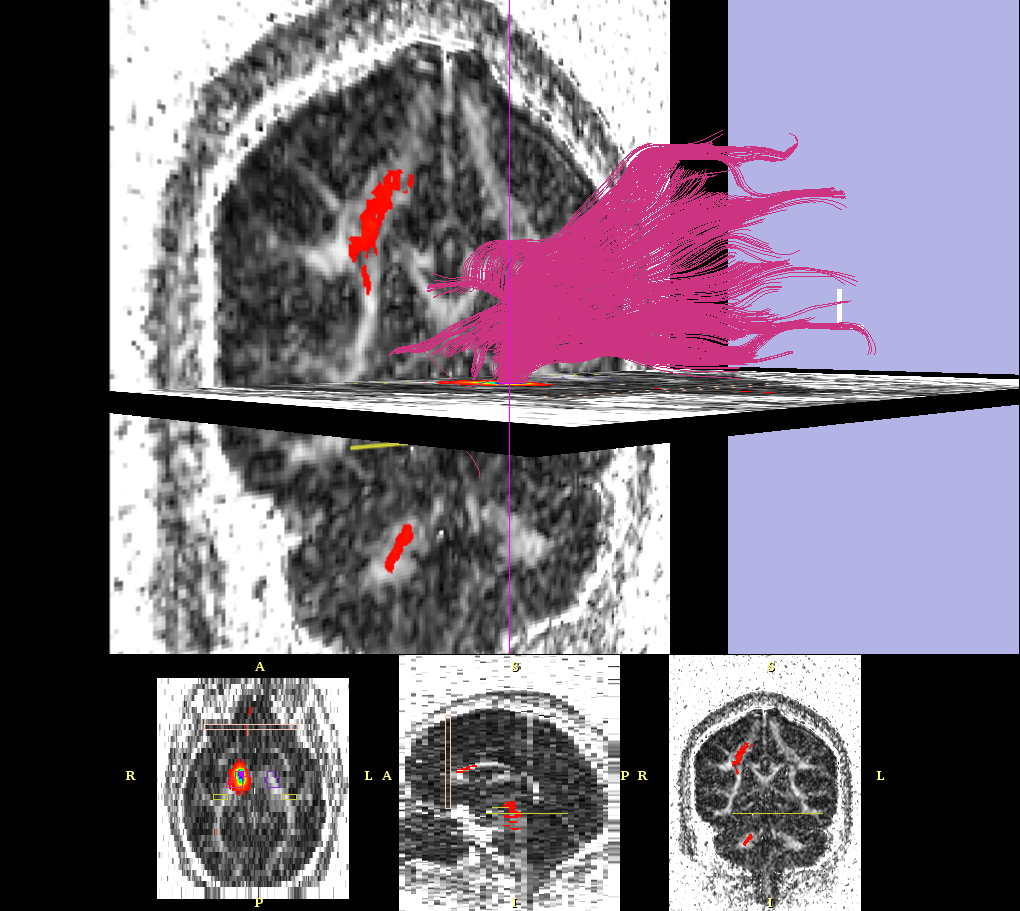
\includegraphics[width=0.5\linewidth]
	  {slicer-0018}
	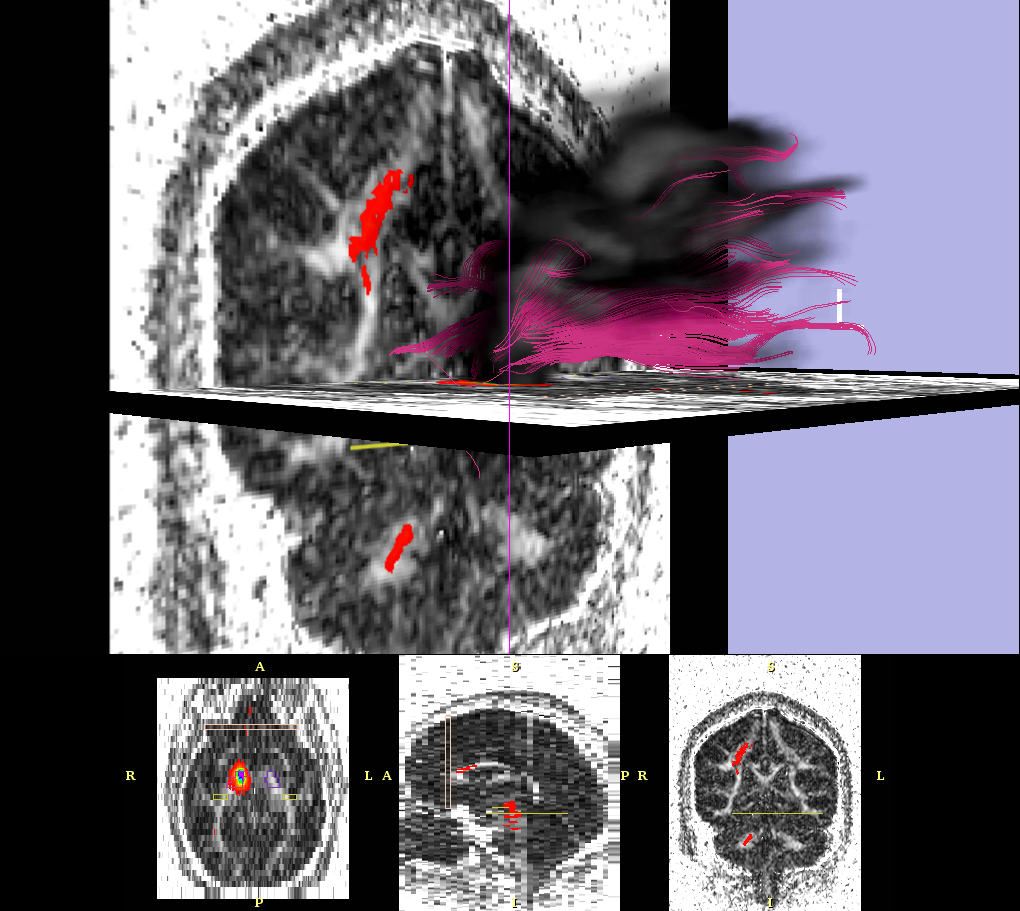
\includegraphics[width=0.5\linewidth]
	  {slicer-0017}
	\caption{On left: Tracts generated using a streamlining method.  On Right: The connectivity map visualized using volume texture rendering overlaid on the streamline generated tracts.  While the two results are similar there are some key differences.Notice that there are regions where there is nonzero probability of connectivity which no tracts from the stream line method pass though.  Also notice that there are regions which have manny streamlines but which the stochastic tractography algorithm predicts is weakly connected. }
\end{figure}

\begin{table} \label{tab:performance}
  \begin{tabular}{ccc}
    \hline & Mean Tract-Average FA & Mean Tract Length (mm)\\
    \hline Stochastic Tractography & 0.4612 & 82.3188 \\
    Streamline Tractography & 0.36859 & N/A\\
    \hline
  \end{tabular}
  \caption{Streamlining results are from research by Gudrun Rosenberger}
\end{table}

\section{Performance}

\begin{figure} \label{fig:performance}
  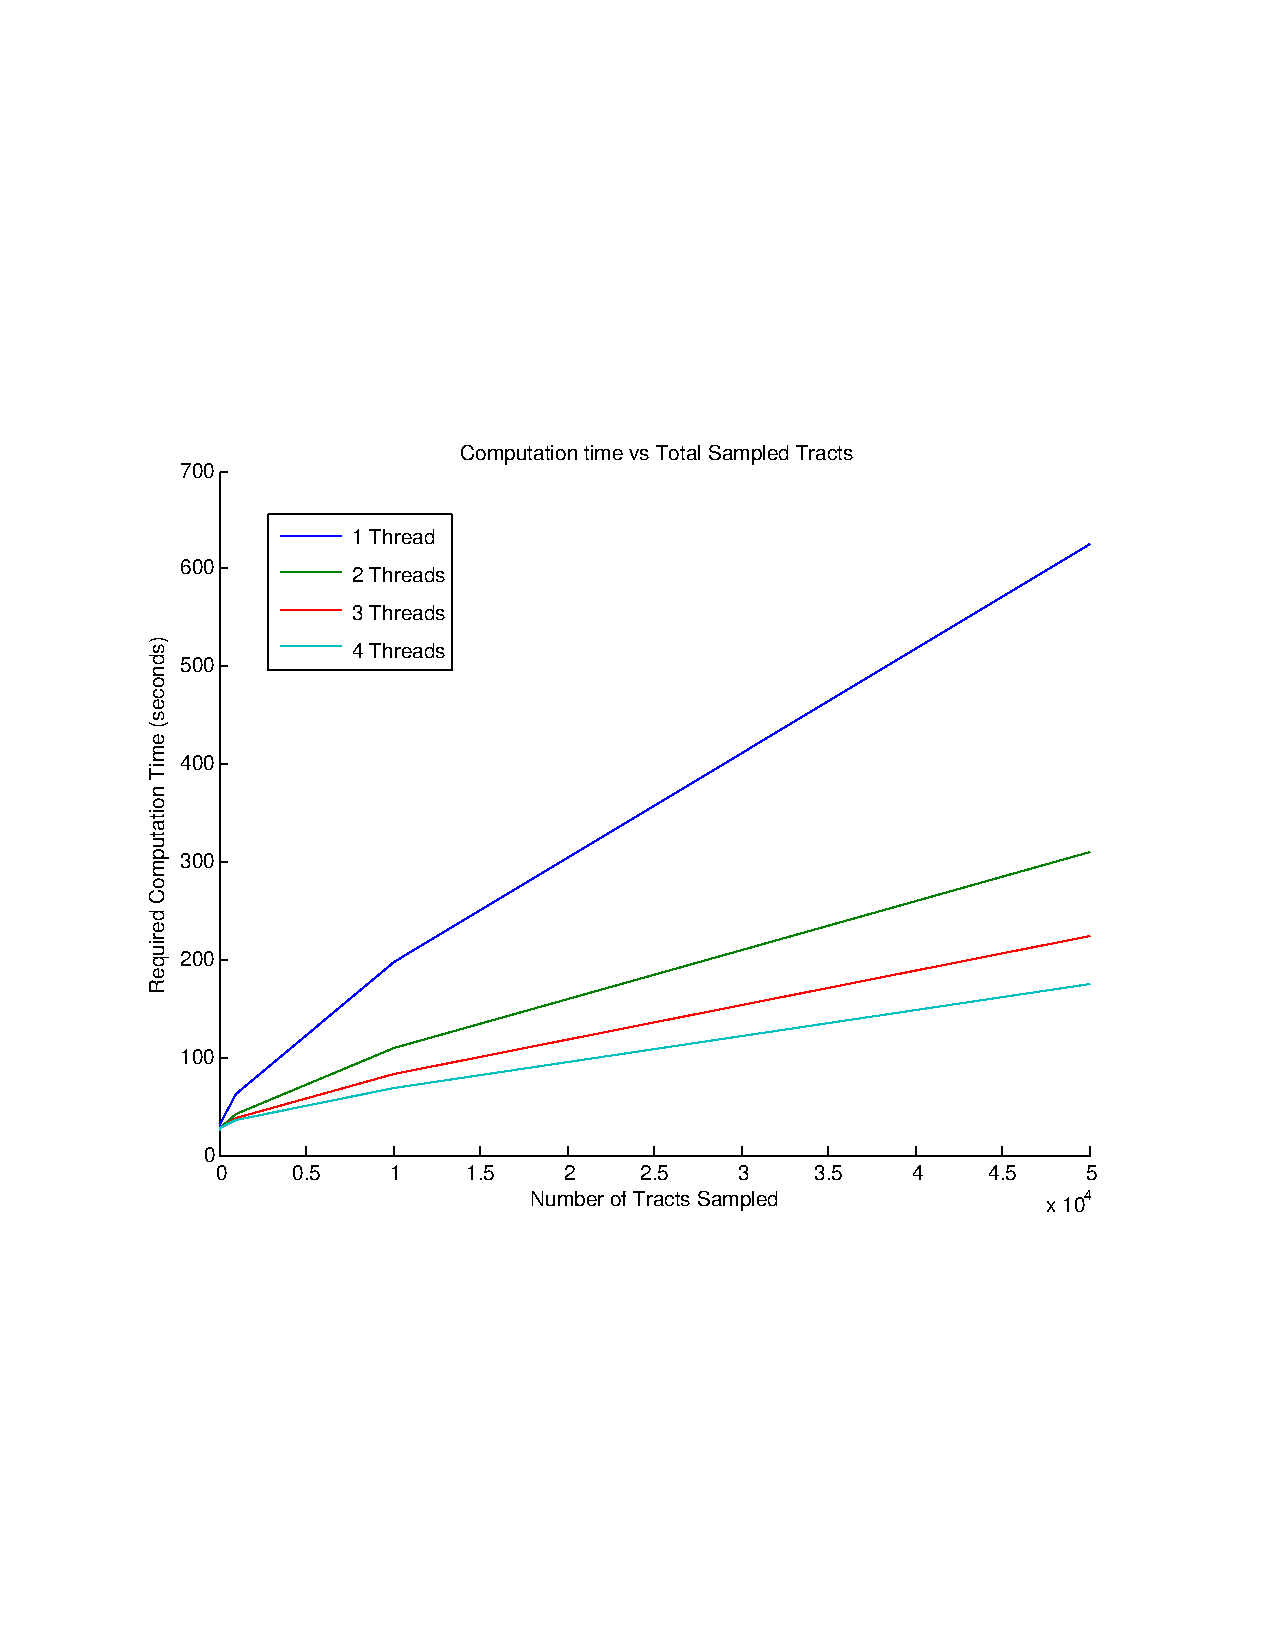
\includegraphics[trim = 20mm 70mm 20mm 70mm, clip, width=0.5\linewidth]
	  {timepertracts}
	\caption{A graph displaying the amount of time needed to sample a number of tracts.  Each line represents the algorithms performance using different numbers of threads.  This test was run on an 8 processor machine.}
\end{figure}
%show tracking in various regions, show correllation with anatomical figures
%show tracking with and without white matter posterior probability map

%show performance improvement with increasing threads
%show performance wrt increasing tract number.
